\section{Background theory}

Digital (and analog) camera sensors can't capture different colors directly.
The way to capture a color picture is to use differently colored filters, which
each let through certain wavelengths of light. Usually the wavelengths
corresponding to the primary colors red, green and blue are used. The first
color pictures were captured by taking three different pictures, each with a
different filter. This is of course slower than taking only one picture, so
digital cameras use a Bayer Filter~\cite{wiki:bayer_filter}.

\begin{figure}[H]
  \centering
  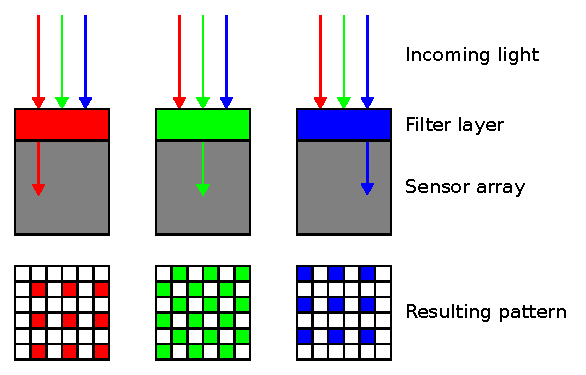
\includegraphics[width=0.8\linewidth]{wiki_bayer}
  \caption{A concept illustration of the Bayer filter~\cite{wiki:bayer_filter}}
\label{fig:wiki_bayer_filter}
\end{figure}

As seen in figure~\ref{fig:wiki_bayer_filter}, the problem with the Bayer
filter is that every pixel only has one color. Every square of four pixels has
1 red, 1 blue and 2 green pixels. To get a proper picture out this data, the
missing two color channels have to be interpolated for each pixel. There are
different interpolation methods, three of which are implemented in this lab
assignment.
